% Editable source for audit_decomposition.pdf (pdflatex; pdftoppm -png -r 150 -singlefile).
% Exact decomposition of the published A->B gap on Q0 from the raw receipts (SOURCE_AUDIT.md section 4).
% ln R = ln(rho online / IC online). Values: A, crypto research/n83_evaluation_20261012/records/panel
% (5 matched pairs); B, tier1_github_38523707244 Panel A (8 pairs, medians). Not one-host measurements.
\documentclass[tikz,border=6pt]{standalone}
\usepackage[T1]{fontenc}
\begin{document}
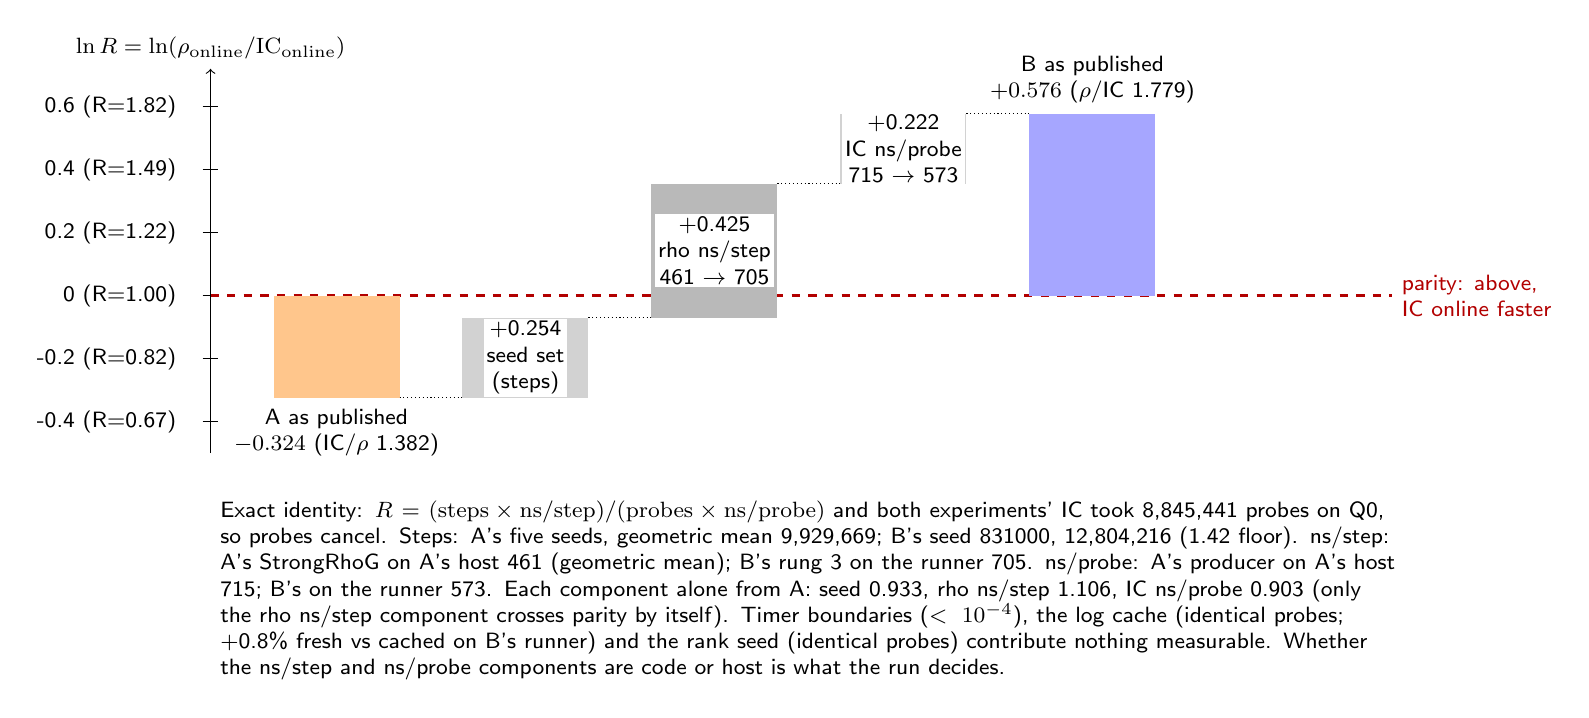
\begin{tikzpicture}[font=\sffamily\footnotesize,x=1mm,y=40mm]
% axis: ln R from -0.5 to 0.7
\def\xa{0}
\draw[->] (0,-0.5) -- (0,0.72) node[above,align=center]{$\ln R = \ln(\rho_{\mathrm{online}}/\mathrm{IC}_{\mathrm{online}})$};
\foreach \v/\r in {-0.4/0.67,-0.2/0.82,0/1.00,0.2/1.22,0.4/1.49,0.6/1.82} {
  \draw (-1,\v) -- (1,\v) node[left=6pt,anchor=east,xshift=-2mm]{\v\ (R=\r)};
}
\draw[red!70!black,thick,dashed] (0,0) -- (150,0) node[right,align=left]{parity: above,\\IC online faster};
% bars
\fill[orange!45] (8,0) rectangle (24,-0.324);
\node[below,align=center] at (16,-0.33) {A as published\\$-0.324$ (IC/$\rho$ 1.382)};
\fill[gray!35] (32,-0.324) rectangle (48,-0.070);
\node[align=center,fill=white,inner sep=1pt] at (40,-0.197) {+0.254\\seed set\\(steps)};
\fill[gray!55] (56,-0.070) rectangle (72,0.355);
\node[align=center,fill=white,inner sep=1pt] at (64,0.143) {+0.425\\rho ns/step\\461 $\to$ 705};
\fill[gray!35] (80,0.355) rectangle (96,0.577);
\node[align=center,fill=white,inner sep=1pt] at (88,0.466) {+0.222\\IC ns/probe\\715 $\to$ 573};
\fill[blue!35] (104,0) rectangle (120,0.576);
\node[above,align=center] at (112,0.58) {B as published\\$+0.576$ ($\rho$/IC 1.779)};
\draw[densely dotted] (24,-0.324) -- (32,-0.324);
\draw[densely dotted] (48,-0.070) -- (56,-0.070);
\draw[densely dotted] (72,0.355) -- (80,0.355);
\draw[densely dotted] (96,0.577) -- (104,0.577);
\node[align=left,anchor=north west,text width=150mm] at (0,-0.62) {Exact identity: $R = (\mathrm{steps}\times\mathrm{ns/step})/(\mathrm{probes}\times\mathrm{ns/probe})$ and both experiments' IC took 8,845,441 probes on Q0, so probes cancel. Steps: A's five seeds, geometric mean 9,929,669; B's seed 831000, 12,804,216 (1.42 floor). ns/step: A's StrongRhoG on A's host 461 (geometric mean); B's rung 3 on the runner 705. ns/probe: A's producer on A's host 715; B's on the runner 573. Each component alone from A: seed 0.933, rho ns/step 1.106, IC ns/probe 0.903 (only the rho ns/step component crosses parity by itself). Timer boundaries ($<10^{-4}$), the log cache (identical probes; +0.8\% fresh vs cached on B's runner) and the rank seed (identical probes) contribute nothing measurable. Whether the ns/step and ns/probe components are code or host is what the run decides.};
\end{tikzpicture}
\end{document}
